\chapter{Transformación canónica infinitesimal y simetría}

	
\begin{tikzpicture}
	\fill [left color=red!50, right color=teal!50] (0,0) rectangle (6.5,.1);
	\fill [left color=teal!50, right color=blue!50] (6.5,0) rectangle (11.5,.1);
	\end{tikzpicture}


\vspace{10mm}
\begin{adjustwidth}{50pt}{50pt}
\begin{ejemplo}

El corchete de Poisson y la transformación canónica infinitesimal nos llevarán al concepto de \emph{generador}, que nos traerá grandes sorpresas. 

\end{ejemplo}
\end{adjustwidth}
\vspace{5mm}
\section{Transformación canónica infinitesimal}
\vspace{5mm}

Empezaremos con un ejemplo para ver de que va todo esto y luego generalizaremos.

\begin{example}

Supongamos un hamiltoniano de la forma:
$\quad H=	\dfrac{p^2_1}{2}+ \dfrac{p^2_2}{2}+\dfrac{q^2_1}{2}+\dfrac{q^2_2}{2}$	

\begin{multicols}{2}

\vspace{2mm}Se trata de una versión simplificada de un oscilador armónico en dos dimensiones.

\vspace{2mm}Tenemos que hacer una transformación canónica que nos viene dada por:

\vspace{2mm}$F_2(q,P,t)=$

$=(q_1P_1+q_2P_2)\cos \theta + (q_1P_2-q_2P_1)\sin \theta $

\vspace{2mm}Como no depende del tiempo, tenemos que $F_2(q,P,t)=F_2(q,P)$

\begin{figure}[H]
	\centering
	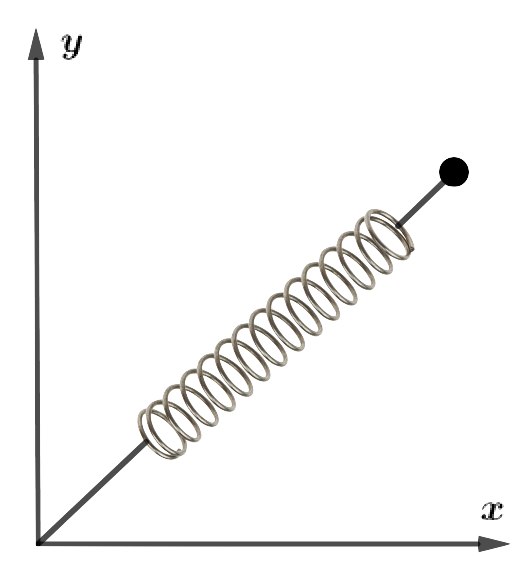
\includegraphics[width=.3\textwidth]{imagenes/img21-01.png}
\end{figure}
\end{multicols}\end{example}

Se puede comprobar que se trata de una transformación canónica, para ello hay que calcular la matriz jacobiana $M$ y comprobar que su determinante es la unidad, $|M|=1$.\footnote{ Comprobación al final del tema}

Empecemos a trabajar a ver qué significa esta transformación. Analizaremos que ocurre si $\theta =0$ y qué ocure cuando $\theta =\varepsilon << 1 \ / \ \varepsilon^2\approx 0$.


\vspace{5mm} $\triangleright\ $ \underline{Análisis $\theta=0$} $\quad \to \quad F_2=q_1P_1+q_2P_2$ Acudiendo a las funciones generadores de transformaciones canónicas del capítulo \ref{T19FG},

$\begin{cases}
\ \displaystyle \pdv{F_2}{q_1}=p_1 & \ \ \displaystyle \pdv{F_2}{q_2}=p_2 \\
\ \displaystyle \pdv{F_2	}{P_1}=Q_1 & \ \ \displaystyle \pdv{F_2}{P_2}=Q_2
\end{cases} \qquad \to \qquad 
\begin{cases}
\ P_1=p_1 & \ \ P_2=p_2	 \\
\ q_1=Q_1 & \ \ q_2=Q_2
\end{cases}$

Se trata de un cambio que no hace absolutamente nada, cambiamos mayúsculas por minúsculas, es como si se tratase de la IDENTIDAD, I, así que en este caso: 
$\quad F_2=q_1P_1+q_2P_2=I$, IDENTIDAD.

\vspace{5mm} $\triangleright\ $ \underline{Análisis $\theta =\varepsilon$} $\  << 1 \ / \ \varepsilon^2\approx 0 \quad \to \quad \sin \varepsilon \approx \varepsilon \ ;\quad \cos \varepsilon \approx 1\ $ \textcolor{gris}{(Taylor)}. La transformación será,

$F_2(q,P) \ \approx \ (q_1P_1+q_2P_2) \ + \ (q_1P_2-q_2P_1)\ \varepsilon \approx I \ + \ \text{algo} \cdot \varepsilon$ 


\vspace{5mm} ?`Esta \subrayado{$\text{transformación infinitesimal}$}, $\ F_2(q,P)\approx (q_1P_1+q_2P_2)  +  (q_1P_2-q_2P_1)\ \varepsilon\, \ $ es \subrayado{$\text{canónica}$}?

Aplicando a las funciones generadores de transformaciones canónicas del capítulo \ref{T19FG},

$\begin{cases}
\ \displaystyle \pdv{F_2}{q_1}=p_1 & \ \ \displaystyle \pdv{F_2}{q_2}=p_2 \\
\ \displaystyle \pdv{F_2	}{P_1}=Q_1 & \ \ \displaystyle \pdv{F_2}{P_2}=Q_2
\end{cases} \qquad \to \qquad 
\begin{cases}
\ P_1+P_2 \varepsilon =p_1 & \ \ P_2-P_1\varepsilon =p_2	 \\ \\
\ \boldsymbol{ q_1-q_2 \varepsilon =Q_1} & \ \ \boldsymbol{q_2+q_1 \varepsilon =Q_2}
\end{cases}$

Despejando las $P_i$ en función de las $p_i$, tenemos: 

$\begin{cases} 
\ \boldsymbol{P_1}=\dfrac 1{1+\varepsilon^2} (p_1-\varepsilon p_2) \approx (1-\varepsilon^2)(p_1-\varepsilon p_2) \approx \boldsymbol{p_1-\varepsilon p_2} \\ \\
\ \boldsymbol{P_2}=\dfrac 1{1+\varepsilon^2} (p_2+\varepsilon p_1) \approx (1-\varepsilon^2)(p_2-\varepsilon p_) \approx \boldsymbol{p_2+\varepsilon p_1}
\end{cases}$

Donde hemos usado que la aproximación de Taylor para $\ f(x)=\dfrac {1}{1+x} \ \ \begin{matrix}  _\approx \\ \begin{tiny}^{x\to 0 }\end{tiny} \end{matrix} \ \ 1-x \ \to \ \dfrac 1{1+\varepsilon^2} \approx 1-\varepsilon^2$

Para pasar de $p_i, \ q_i$ a $P_i,\ Q_i$ tenemos:
$\quad\begin{cases} 
\ \boldsymbol{ q_1- \varepsilon q_2 =Q_1} & \quad \boldsymbol{q_2+ \varepsilon q_1=Q_2}	\\ \\
\ \boldsymbol{p_1-\varepsilon p_2 \approx P_1} & \quad \boldsymbol{p_2+\varepsilon p_1 \approx P_2}
\end{cases}$

Construyamos la matriz jacobiana $M$, que ahora será $4 \times 4$,


$M\ = \ \mqty(
\pdv{Q_1}{q_1} & \pdv{Q_1}{q_2} & \pdv{Q_1}{p_1} & \pdv{Q_1}{p_2} \\
\pdv{Q_2}{q_1} & \pdv{Q_2}{q_2} & \cdots & \cdots \\
\cdots & \cdots & \pdv{P_1}{p1} & \cdots \\
\cdots & \cdots & \cdots & \pdv{P_2}{p_2}
) \ = \ 
\mqty(
1&-\varepsilon & 0 & 0 \\ \varepsilon & 1 & 0 & 0 \\ 0 & 0 & 1 & -\varepsilon \\ 0 & 0 & \varepsilon & 1 
)$

Calculemos el determinante por Laplace, adjuntos de la primera columna,

$|M| \ = \ 
1 \ (-1)^{1+1} \ \mqty| 1&0&0 \\ 0&1&-\varepsilon \\ 0 & \varepsilon & 1  | + 
\varepsilon \ (-1)^{2+1} \ \mqty| -\varepsilon & 0 & 0 \\ 0 & 1 & - \varepsilon \\ 0 & \varepsilon & 1 |    
= (1+\varepsilon^2) - \varepsilon (-\varepsilon - \varepsilon^3 )   \approx 1     \,  , \ $ a orden $\varepsilon$.


Luego, la transformación infinitesimal, $\ F_2(q,P)\approx (q_1P_1+q_2P_2)  +  (q_1P_2-q_2P_1)\ \varepsilon\ = I + \varepsilon \text{ algo} , \ $ es canónica a orden $\varepsilon$.


A este $\text{algo}$ le vamos a llamar \text{\emph{generador}} de la transformación canónica infinitesimal, $\ G: \ F_2=I+\varepsilon G$ 

$\boldsymbol G\ = \ q_1P_2\ - \ q_2P_1 \ \ $
Si sustituimos $P_1$ y $P_2$ por las aproximaciones encontradas para $\varepsilon <<1$, tenemos:

$G=q_1(p_2+\varepsilon p_1)-q_2(p_1-\varepsilon p_2)=q_1p_2-q_2p_1+\varepsilon( \cdots ) \ \ $


Como $F_2=I+\varepsilon G  \to $ al sustituir obtenemos un término en $\varepsilon^2 \approx 0$ que despreciamos  y trabajaremos con el siguiente generador:
$\quad \boldsymbol G\ = \ q_1p_2\ - \ q_2p_1$

\vspace{5mm} Se tiene el siguiente \textbf{teorema}:

$$\text{Si }\  G \ \text{ genera una simetría continua en el hamiltoniano}  \ \Leftrightarrow \ \{G,H\} \ = 0$$

Teorema que nos proporciona una manera de descubrir si el hamiltoniano posee o no una simetría.

\underline{Comprobación}:

Volvamos al ejemplo de nuestro Hamiltoniano, $\ H=\dfrac {p_1^2} 2 + \dfrac {p_2^2} 2 + \dfrac {q_1^2} 2 + \dfrac {q_2^2} 2 \, , \  $ con $\ G=p_1q_2-q_2p_1 \ $ y calculemos el corchete de Poisson $\ \{G,H\}\, :$


$\{G,H \} = \{ p_1q_2-q_2p_1, H\} = \{q_1p_2,H\}-\{q_2p_1,H\}= q_1\{p_2,H\} + \{q_1,H\}p_2 - q_2\{p_1,H\} - \{q_2,H\}p_1 $

Tengamos en cuenta las propiedades vistas en el tema anterior: $\ \{q,p\}=1;\ \{q,q\}=0;\ \{p,p\}=0\, ,$ que se puede demostrar que generalizadas dan lugar a $ \  \boldsymbol{ \{q_i,q_j\}=0;\ \{p_i,p_j\}=0;\ \{q_i,P_j\}=\delta_{ij} } \, , \ $  siendo $ \ \delta_{ij} \ $ el delta de Kronecker. 

Sustituyamos $\ H=\dfrac {p_1^2} 2 + \dfrac {p_2^2} 2 + \dfrac {q_1^2} 2 + \dfrac {q_2^2} 2\ $ y calculemos, uno a uno, los cuatro corchetes de Poisson que acabamos de obtener:

\begin{itemize}
\item $\ \{p_2,H\}= \left\{p_2\ , \ \dfrac {p_1^2} 2 + \dfrac {p_2^2} 2 + \dfrac {q_1^2} 2 + \dfrac {q_2^2} 2 \right\} \ = \ 0 \ + \ 0 \ + \ 0 \ + \left\{p_2,\dfrac{q_2^2}2 \right\} \ = \ - \left\{\dfrac{q_2^2}2 , p_2 \right\}  \ = \ -\dfrac {q_2^2}{2} \ \{p_2\; q_2, q_2\}  -\dfrac 1 2 \left[ q_2 \ \cancelto{1}{ \{q_2,p_2\} } + \cancelto{1}{ \{q_2,p_2\} } q_2 \right] = -\dfrac 1 2 [q_2+q_2] \ = \ \textcolor{red}{-q_2}$	
\item $\{q_1,H\}=\left\{q_1\ , \ \dfrac {p_1^2} 2 + \dfrac {p_2^2} 2 + \dfrac {q_1^2} 2 + \dfrac {q_2^2} 2 \right\} \ = \ \left\{q_1,\dfrac{p_1^2}2 \right\} \ + \ 0 \ + \ 0 \ + \ 0  \ = \ - \dfrac 1 2  \left\{p_1\ p_1 , q_1 \right\}  \ = \ -\dfrac 1 2 [\ p_1\{p_1,q_1\} + \{p_1,q_1\}p_1 \ ] \ =  \ -\dfrac 1 2 \left[- \ p_1 \ \cancelto{1}{\{q_1,p_1\}} -  \cancelto{1}{\{q_1,p_1\}}p_1 \ \right]=\ \textcolor{red}{p_1} $
\item Análogamente, $\quad \{p_1,H\}\ = \ \left\{ p_1,\dfrac{q_1^2}{2} \right\}\ = \ \textcolor{red}{-q_1} \ $ y también  $ \ \{q_2,H\} \ = \ \textcolor{red}{p_2}$
\end{itemize}

Volviendo a la expresión del corchete de Poisson,
$\quad \{G,H\}\ = \ -q_1 \textcolor{red}{q_2} \ + \ \textcolor{red}{p_1} p_2 \ + \ q_2 \textcolor{red}{q_1} \ - \ p_1 \textcolor{red}{q_2} \ = \ 0$


Como $\dot f=\{f,H\}+\displaystyle \pdv{f}{t}$ y nuestra $f=G=q_1p_2-q_2p_1=G(q,p)\neq G(t)$, entonces, 

$\ \dot G=\displaystyle \dv{G}{t} =\cancelto{0}{\{G,H\}} + \displaystyle \cancelto{0}{\pdv{G}{t}} = 0 \ \to \ G \ $ es una constante del movimiento.


Además, genera una transformación que, como comprobaremos a continuación, deja invariante el hamiltoniano, por lo que se tratará de una transformación de \emph{simetría}.

--- Hamiltoniano: $ \ H \ = \ \ \dfrac {p_1^2} 2 + \dfrac {p_2^2} 2 + \dfrac {q_1^2} 2 + \dfrac {q_2^2} 2$

--- Transformación canónica infinitesimal para pasar de $p,q$ a $Q,P$, como hemos hecho anteriormente (hay que despejar $q(Q) \to  \quad \ \begin{cases} \ q_1=Q_1+\varepsilon Q_2 & \quad p_1=P_1+\varepsilon P_2 \\ \ q_2=Q_2-\varepsilon Q_1 &\quad p_2=P_2-\varepsilon P_1 \end{cases}$

\begin{footnotesize} \textcolor{gris}{Hemos usado la misma aproximación anterior $\left( \dfrac 1{1+\varepsilon^2}\approx  1-\varepsilon^2 \right)$ } \end{footnotesize}

Transformemos nuestro hamiltoniano:

$\widetilde H =\dfrac 1 2 \left[ (P_1+\varepsilon P_2)^2 + (P_2-\varepsilon P_1)^2 + (Q_1+\varepsilon Q_2)^2 + (Q_2-\varepsilon Q_1)^2 \right] =$

$=\dfrac 1 2 \left[ P_1^2 + \varepsilon^2 P_2^2 +\cancel{ 2 \varepsilon P_1 P_2} + P_2^2 + \varepsilon^2 P_1^2 -\cancel{ 2 \varepsilon P_1 P_2} +
	 Q_1^2 + \varepsilon^2 Q_2^2 +\bcancel{ 2 \varepsilon Q_1 Q_2}  +
	 Q_2^2 + \varepsilon^2 Q_1^2 -\bcancel{ 2 \varepsilon P_1 P_2} \right]=$
	 
$=\dfrac 1 2 [ \ (1+\varepsilon^2)P_1^2+ (1+\varepsilon^2)P_2^2+(1+\varepsilon^2)Q_1^2+(1+\varepsilon^2)Q_2^2 \ ] = (1+\varepsilon)^2 \widetilde H = \ \text{ (a orden } \varepsilon) \ = \widetilde H \ = \ H$

Luego, el hamiltoniano es invariante, a orden $\varepsilon$, para la transformación infinitesimal.

\begin{center} \rule{250pt}{0.1pt} \end{center}

Volvamos a nuestra \subrayado{$\text{transformación canónica \emph{finita}}$} $\ F_2(q,P)=(q_1P_1+q_2P_2)\cos \theta + (q_1P_2-q_2P_1)\sin \theta \ $ y vamos a probar que deja invariante al hamiltoniano.

Aplicando las ecuaciones de transformación de las funciones $F_2$, capítulo \ref{T19FG}, tenemos:


$\begin{cases} \ \displaystyle \pdv{F_2}{q_1} = p_1; &\ \ \displaystyle  \pdv{F_2}{q_2}=p_2 \\  \ \displaystyle \pdv{F_2}{P_1} = Q_1; &\ \ \displaystyle  \pdv{F_2}{P_2}=Q_2 \end{cases} \quad \longrightarrow \quad 
\begin{cases}
\ p_1=P_1\cos \theta + P_2 \sin \theta ; &\ \ \ 	p_2=P_2\cos \theta - P_1 \sin \theta \\ \ Q_1=q_1\cos \theta - q_2 \sin \theta ; &  \ \ \ Q_2=q_2\cos \theta + q_1 \sin \theta
\end{cases}$

Despejando las $q$ en función de las Q, tendremos: $\quad q_1=Q_1\cos \theta + Q_2 \sin \theta ;\ \ q_2=-Q_1\sen \theta + Q_2 \cos \theta$

\textcolor{gris} {La matriz de cambio de $Q\to q$ es  $\mqty(c&-s\\s&c)$, de determinante $1$ y ortogonal $\left( \mqty(c&s)\mqty(-s\\c)=0 \right)$, por lo que su inversa coincide con la traspuesta, $\mqty(\ )^{-1}=\mqty(\ )^T$, lo que facilita mucho el cálculo.}


Al sustituir en el hamiltoniano, 

$p_1^2+p_2^2=P_1^2 \cos^2 \theta + P_2^2 \sin^2 \theta + \cancel{2P_1P_2\cos \theta \sin \theta} + P_2^2 \cos^2 \theta + P_1^2 \sin^2 \theta -\cancel{2P_1P_2\cos \theta \sin \theta}=P_1^2+P_2^2$

Análogamente, $º q_1^2+q_2^2=Q_1^2+Q_2^2$, por lo que $\widetilde H=\dfrac 1 2 (P_1^2+P_2^2+Q_1^2+Q_2^2)=H$, luego $H$ es invariante bajo la transformación $F_2$.


\vspace{5mm} Volvamos a enunciar el teorema anterior en la forma: 

\begin{large}
\begin{theorem}

\vspace{2mm} Si $\ F_2\ $, función generadora de una transformación canónica, se puede expresar como $	\ \displaystyle F_2 \ = \ \sum_{i=1}^n q_iP_i \ + \ \varepsilon \ G \, \ $ con $\ G\neq G(t)\ $ y con $\ \{G,H\}\ = \ 0 \ $

\vspace{4mm} \hspace{2cm} entonces, 

\vspace{4mm} $G\ $ es una \emph{magnitud conservada} y, además, genera una \emph{simetría continua} del $\ H.$
\end{theorem}
\end{large}

\rule{200pt}{0.1pt}

\vspace{5mm} Para el hamiltoniano del \emph{oscilador isotrópico en 2-dim},
$\ H=\dfrac{p_x^2}{2m}+\dfrac{p_y^2}{2m}+\dfrac{m\ \omega^2}{2} \ (x^2+y^2)\, , \ $
se tiene que $\ G=q_1p_2-q_2p_1= \ xp_y-yP_x \ = \ L_z \ = \ \text{constante} \ $ se conserva la componente $z$ del momento angular y es el propio momento angular quien genera la simetría.

\vspace{1.5cm}
\color{NavyBlue}
\begin{ejercicio}
	\textcolor{NavyBlue}{Comprobación que la transformación dada $\ F_2(q,P) \ $ es canónica, para ello calcularemos el jacobiano, $M$, y comprobaremos que su determinante es $1$.}
\end{ejercicio}



\vspace{5mm}

$F_2(q,P,t)(q_1P_1+q_2P_2)\cos \theta + (q_1P_2-q_2P_1)\sin \theta $

Ecuaciones de la función de generadoras, capítulo \ref{T19FG},

$\begin{cases}
\ \displaystyle \pdv{F_2}{q_1}=p_1 & \ \ \displaystyle \pdv{F_2}{q_2}=p_2 \\
\ \displaystyle \pdv{F_2	}{P_1}=Q_1 & \ \ \displaystyle \pdv{F_2}{P_2}=Q_2
\end{cases} \qquad \to \qquad 
\begin{cases}
\ Q_1=q_1\cos \theta - q_2 \sin \theta & \ \ Q_2=q_2\cos \theta+q_1\sin \theta \\
\ p_1=P_1 \cos \theta +P_2 \sin \theta & \ \ p_2=P_2\cos \theta - p_1 \sin \theta 
\end{cases}$

Necesitamos escribir las $P$ en función de la $p$, de lo anterior,

$\mqty(p_1\\p_2)=\mqty(\cos \theta & \sin \theta \\-\sin \theta & \cos \theta) \mqty(P_1 \\ P_2) \ \to  \ p=C\ P \quad \text{ con } \ C= \mqty(\cos \theta & \sin \theta \\-\sin \theta & \cos \theta) $

Como $\ |C|=1 \ $ y $C$ es ortogonal, $\left( \  \mqty(\cos \theta \\ -\sin \theta)^T \ \mqty(\sin \theta \\ \cos \theta)=
\mqty(\cos \theta & -\sin \theta) \ \mqty(\sin \theta \\ \cos \theta)=0 \ \right) \, , $ por lo que $\ C^{-1}=C^T\, , \ $ luego,

$p= C \ P \ \to \ P= C^{-1} p = C^T p =\mqty(\cos \theta & -\sin \theta \\ \sin \theta & \cos \theta ) \mqty(p_1\\p_2) \ \to \ \begin{cases} \ P_1=p_1 \cos \theta - p_2 \sin \theta \\ \ P_2= p_1\sin \theta + p_2 \cos \theta \end{cases}$

Con las relaciones, $\ \begin{cases}\ Q_1=q_1\cos \theta - q_2 \sin \theta \\ \ Q_2=q_2\cos \theta+q_1\sin \theta    \end{cases} \ $ y $ \quad  \begin{cases} \ P_1=p_1 \cos \theta - p_2 \sin \theta \\ \ P_2= p_1\sin \theta + p_2 \cos \theta \end{cases}\ \ $ formamos $M$:



$M\ = \ \mqty(
\pdv{Q_1}{q_1} & \pdv{Q_1}{q_2} & \pdv{Q_1}{p_1} & \pdv{Q_1}{p_2} \\
\pdv{Q_2}{q_1} & \pdv{Q_2}{q_2} & \cdots & \cdots \\
\cdots & \cdots & \pdv{P_1}{p1} & \cdots \\
\cdots & \cdots & \cdots & \pdv{P_2}{p_2}
) \ = \ 
\mqty(
\cos \theta & - \sin \theta & 0 & 0 \\ 
\sin \theta &  \cos \theta & 0 & 0 \\
0& 0& \cos \theta & - \sin \theta \\
0& 0& \sin \theta &  \cos \theta
)\ \, \ \ $ que calculando el determinante con cualquier sw. adecuado (o por adjuntos de Laplace de cualquiera de lus filas o columnas) se obtiene que $\ |M| = 1 \hspace{14cm} \Box$


\color{Black}

